\chapter{Introduction}
\label{intro} 

Modern integrated systems and other programmable electronics often have safety-measures built in to avoid unintended behaviour, whether it be accidental or intentional, from an external source. These safety measures typically only address software or firmware issues, leaving systems unprotected against hardware-induced faults, known as glitch attacks. These attacks are able to bypass robust software and firmware security measures given the right method of attack. Interestingly, despite the importance of glitch protection, it only started gaining attention after practical glitch attacks first made their appearance in 2002 through an optical fault attack\cite{trouchkine2019fault}. 

In the world of computer architecture, many aspects remain closely guarded secrets, including preventive measures against glitch attacks. This secrecy often makes these preventative measures inaccessible to the public. Over recent years there has been a large shift away from this secrecy as more and more researchers and companies use the \textit{RISC-V} instruction set architecture (ISA)\cite{riscv_manual}. This architecture is open source, allowing anyone with the right knowledge and motivation to create their own central processing unit (CPU). One group of people doing this is the \textit{OpenHW Group} who have developed several publicly available RISC-V CPUs over recent years. One of these is the CV32E40S, which is a core mainly focused on safeguarding against glitch- and side-channel attacks\cite{cv32e40s_manual}.

While the CV32E40S has proven to be able to detect glitch attacks, it comes at a cost in performance. Often the methods used to protect against attacks are complex and increase the execution time and power needed for the CPU to perform its given tasks. In addition, these methods only cover specific parts of the core while leaving other pars exposed. This project investigates the possibility of replacing some of the security features of the CV32E40S in favour of running two CPUs in a \textit{Dual-Core Lockstep} (DCL) mechanism instead to increase throughput, simplicity and fault detection coverage. Henceforth the core using the DCL mechanism is referred to as the CV32E40DC. 

\section{Sustainability}
\label{sec:sustainability}

Out of the 17 sustainability goals of the United Nations\cite{un}, at least two can be considered highly relevant for this project. 

\begin{itemize}
    \item \textbf{Goal 9:} Build resilient infrastructure, promote sustainable industrialization and foster innovation.
    \item \textbf{Goal 17:} Revitalize the global partnership for sustainable development.
\end{itemize}

The goal of this project is to investigate a new way of possibly making components more resilient against attacks and exploits. In turn this will also make the devices of normal consumers less susceptible to attacks, which might benefit society as a whole. This fits into \textit{goal 9}. In addition, this project works to increase the knowledge around an open source project. Being open source means anyone in the world can access all parts of the code. This is relevant for promoting \textit{goal 17} of revitalizing global partnership for sustainable development. 

\section{The use of AI}
\label{sec:AI}

The AI chat bot ChatGPT made by \textit{Open AI}\cite{chat} was used as an academic tool when working on this project. Its main use was to offer inspiration for possible ways to restructure parts of the text that could be difficult to understand or where the point did not come across clearly. \autoref{fig:chatGPT} shows a typical use of ChatGPT.

\begin{figure}[h!]
    \centering
    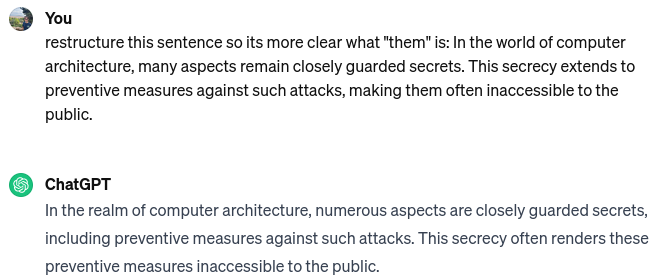
\includegraphics[width=0.8\textwidth]{docs/images/chat_gpt_use.png}
    \caption{Typical use of ChatGPT.}
    \label{fig:chatGPT}
\end{figure}

In this project it was also used to write the code shown in \autoref{lst:dc_code}. This is SystemVerilog code where modules with large interfaces are instantiated and a lot of signals that are copies of preexisting ones are made with the added suffix "\_cmp" or "\_reg". This is code that is very repetitive and writing it can therefore be significantly sped up with the help of AI

\section{Source code}

All source code for this project can be found at the \href{https://github.com/JarlMS/Dual-RISCV-core-for-glitch-protection}{Dual RISC-V core for glitch protection} Github repository\footnote{https://github.com/JarlMS/Dual-RISCV-core-for-glitch-protection}.

